To complement the LSD localizer, which returns a line segment in the middle of
the barcode (hereafter called \emph{best line}), we need to find the barcode's boundaries before we can attempt to read it.

\subsection{Variation}
The variation boundary finder is the original boundary detection method proposed
in \cite{Creusot2016} in conjunction with the LSD localization. Let $L_\perp$
denote the sequence of intensity values along the line perpendicular to the best
line, going through the best line's center (hereafter called \emph{bisector}).
Since barcodes consist of alternating black and white bars, the variation of
intensity values along a line crossing the barcode is expected to be high. The
boundary points are thus expected to have the following property: Extend a 
``probing'' line (\emph{inner probe}) from the boundary point along the bisector, pointing inside the
barcode, i.e. in direction of best line's center. Extend a second ``probing''
line (\emph{outer probe}) from the boundary point in the opposite direction, away from the barcode.
The variation along the inner probe is now expected to be much higher than the
variation along the outer probe.

To find the boundary points, for each index $k$ along the bisector, the signed variation
difference
\begin{equation*}
 \phi_{L_\perp} (k)=\sum_{j=-R}^{0}\abs{L_\perp(k+j)-L_\perp(k+j-1)}-\sum_{j=0}^{R}\abs{L_\perp(k+j)-L_\perp(k+j+1)}
\end{equation*}
is computed. Here, $R$ is the probing distance, which we chose as $R=l_*/2$,
half of the length of the best line.

The right boundary point should lie at the
bisector index with maximal $\phi_{L_\perp}$, while the left boundary point
should have minimal $\phi_{L_\perp}$.

We deviate slightly from \citeauthor{Creusot2016} by instead using the variation
measure
\begin{equation*}
 \phi_{L_\perp}^* (k)=\sum_{j=-R}^{0}\abs{L_\perp(k+j)-L_\perp(k+j-1)}\cdot (R+j)-\sum_{j=0}^{R}\abs{L_\perp(k+j)-L_\perp(k+j+1)}\cdot (R-j)\,,
\end{equation*}
giving higher weight to pixel values near the current boundary candidate at
index $k$.

\subsection{LSD Bound}
Motivated by the high quality of line segments returned by LineSegmentDetector,
we constructed a new boundary finder, using ideas from the variation method
described above. The goal is to determine the line segments corresponding to the two
outer barcode bars, the \emph{boundary segments}.

We first filter the line segments, so that only segments parallel to and located
next to the best
line are kept. To that end, we use the angle criterion and the criterion of sufficient
projected intersection as described in \cref{sec:LSD}. The remaining segments
are sorted based on the position of the projection of their centers onto the
bisector line. The boundary segments should have the following property: As before,
extend an inner probe from the projected center of the boundary segment along the bisector, pointing inside the
barcode. Extend an outer probe in the opposite direction, away from the barcode.
The inner probe is expected to cross a large number of line segments parallel to
and located next to the best line (i.e. segments which have not been
filtered out in the previous step). The outer probe is expected to cross fewer
such lines.
...

\subsection[Wachenfeld]{Wachenfeld}
Another implementation was adapted from the barcode detection and recognition algorithms proposed by Wachenfeld et al. \cite{wachenfeld2008robust}. The method is subdivided into the three steps of preprocessing, barcode edge detection and hypothesis based reading. Since we implemented barcode localization (\cref{sec:Localization}) and barcode reading (\cref{sec:Reading}) as separate steps only the edge detection with a bit of preprocessing is adapted.

The originally proposed boundary detection assumes that the position of the barcode is centered. This way a simple scan line can be applied to the picture. If the barcode is unreadable or misaligned the scan line can be reapplied with a rotation or shift factor. Since the position and rotation of the barcode is already determined in the localization step it is sufficient to place a scan line perpendicular to the best line. To simplify further steps we applying a affine transformation to the region around the scan line.

For the preprocessing we need to first detect to local maxima and minima. Our pictures are already converted to gray scale on loading so we can directly traverse the scan line from to middle pixel toward the outside and look for neighboring pixels with difference in value greater then a set threshold. In a second step we need to remove overly extreme points by executing a pruning step. Lastly we need to apply a dynamic threshold by always comparing every local extrema to an inwards neighborhood.

The boundary detection is based on some properties of the barcode. As shown in \cref{sec:Intro} a EAN13 barcode consist of 95 alternating black and white lines. These lines can only be arranged based on the 20 patterns defined by the specification. The patterns also have the property that every patter has exactly 4 alternations. This means a full barcode has 59 segments of black and white: 2 $\times$ 3 for the outer guard, 5 for the inner guard and 12 $\times$ 6 for the 12 digits.

To detect the boundaries we start with the middle pixel. If this pixel is white we look for the nearest black pixel. The corresponding black segment of this pixel is selected. From this selection we traverse toward the outsides by looking for the smallest neighboring pair of white and black segments to the left and right and adding it to the current selection. The selected region must be at all times be enclosed by black segments. This process is demonstrated in \cref{wachenfeld}. The smallest pair of segments is required to prevent the algorithm from selecting the quit zone.

The outer guard bars are detected as soon as we have selected all 59 black and white segments respectively 29 pairs and the initial middle segment.

\begin{figure}[t]
\center
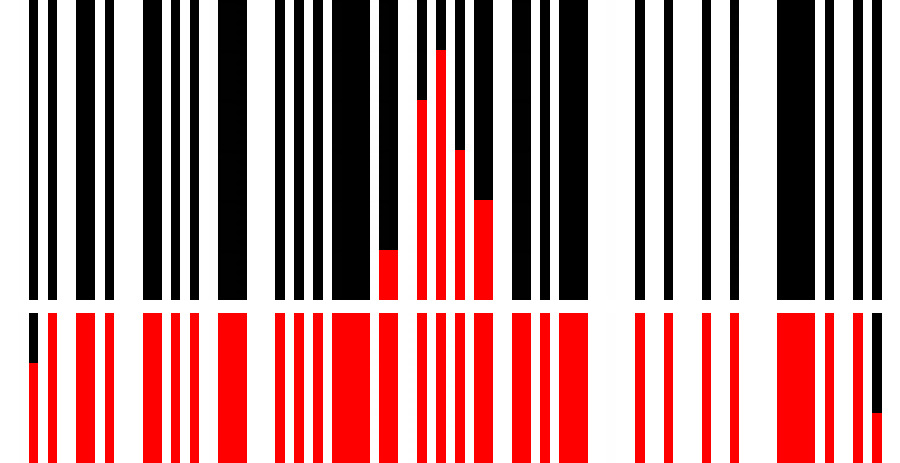
\includegraphics[width=0.6\textwidth,natwidth=900,natheight=463]{img/wachenfeld.png}
\caption{Application of the Wachenfeld boundary detection. The selection is colored in red. Steps are shown from top to bottom.}
\label{wachenfeld}
\end{figure}


%%% Local Variables:
%%% mode: latex
%%% TeX-master: "00Ausarbeitung.tex"
%%% End: